\chapter{初段ミューオントリガー性能評価}
実際にRun-3での性能について書く
位置依存性とか大量に
\section{Run3における初段シングルミューオントリガー}
\subsection{Efficiency}
Date と MC でeffの比較

\subsection{Trigger Rate}
Date と MC
\begin{figure}[tb]
  \centering
  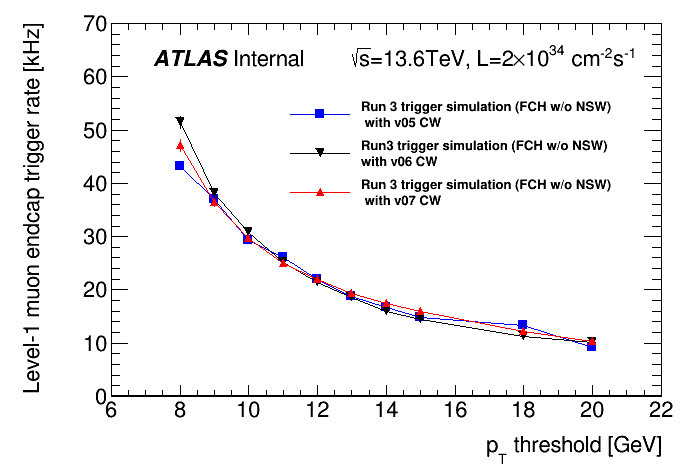
\includegraphics[clip, width=14cm]{fig/5/l1mue_rate_run3.png}
  \caption{Rate}
  \label{fig:fit_def}
\end{figure}

\subsection{電荷}


